%====================================================================
\frame{ \frametitle{Posterior distribution}

  \paragraph{Aim:} Evaluate
  $$
  E[f(\thetabf) | \Ybf]
  $$
  \begin{itemize}
   \item Posterior mean: $f(\thetabf) = \theta_j$
   \item Credibility interval: $f(\thetabf) = \Ibb\{\theta^\ell_j < \theta_j < \theta^u_j\}$
   \item Posterior variance: $f(\thetabf) = \theta_j^2$ \qquad (+ posterior mean)
  \end{itemize}

  \bigskip \bigskip \pause
  \paragraph{Main problem:} evaluate
  $$
  p(\thetabf \gv \Ybf) = \frac{\pi(\thetabf) \bf \ell(\Ybf \gv \thetabf)}{p(\Ybf)}
  $$
  which requires to evaluate
  $$
  p(\Ybf) = \int \underset{prior}{\underbrace{\pi(\thetabf)}} \; \underset{likelihood}{\underbrace{p(\Ybf | \thetabf)}} \d \thetabf
  $$
}

%====================================================================
\subsection{Conjugate priors}
\frame{\frametitle{Outline} \tableofcontents[currentsubsection]}
%====================================================================
\frame{ \frametitle{Nice case: Conjugate priors}

  \paragraph{Example: Bernoulli}\footnote{\#\ref{slide:prior}: from top to bottom, $(a, b) = (1, 10), (5, 5), (1, 1)$}
  \begin{description}
   \item[Prior:] $\theta =$ probability to be sick. 
   $$
   \theta \sim \Beta(a, b), 
   \qquad 
   \pi(\theta) \propto \theta^{a-1} (1-\theta)^{b-1}
   $$ \pause
   \item[Likelihood:] $Y_i = 1$ if sick, $0$ otherwise. $S =$ number of sick
   $$
   Y_i \gv \theta \sim \Bcal(\theta), 
   \qquad 
   \ell(\Ybf \gv \theta) = \prod_i \theta^{Y_i} (1-\theta)^{1-Y_i} = \theta^{S} (1-\theta)^{n-S}
   $$ \pause
   \item[Posterior:]
   $$
   p(\theta \gv \Ybf) \propto \pi(\theta) \ell(\Ybf \gv \theta) = \theta^{a+S-1} (1-\theta)^{b+n-S-1}
   $$
   which means that
   $$
   \theta \gv \Ybf \sim \Beta(a+S, b+n-S)
   $$
  \end{description}
}

%====================================================================
\frame{ \frametitle{Conjugate priors: Discrete distributions}

  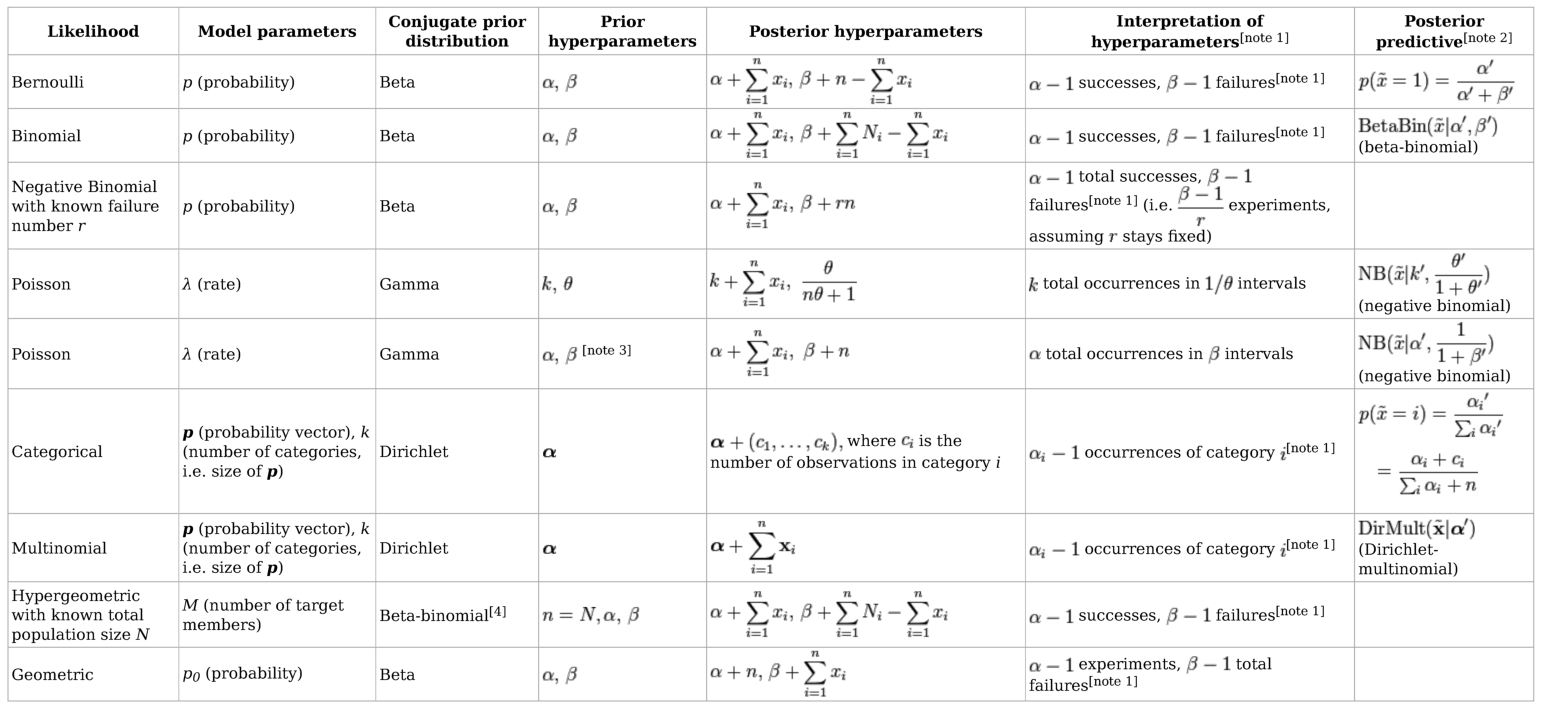
\includegraphics[width=1\textwidth]{../figs/WikipediaConjugatePrior-Discrete}

  \footnotesize{\url{en.wikipedia.org/wiki/Conjugate_prior}}
}

%====================================================================
\frame{ \frametitle{Conjugate priors: Continuous distributions}

  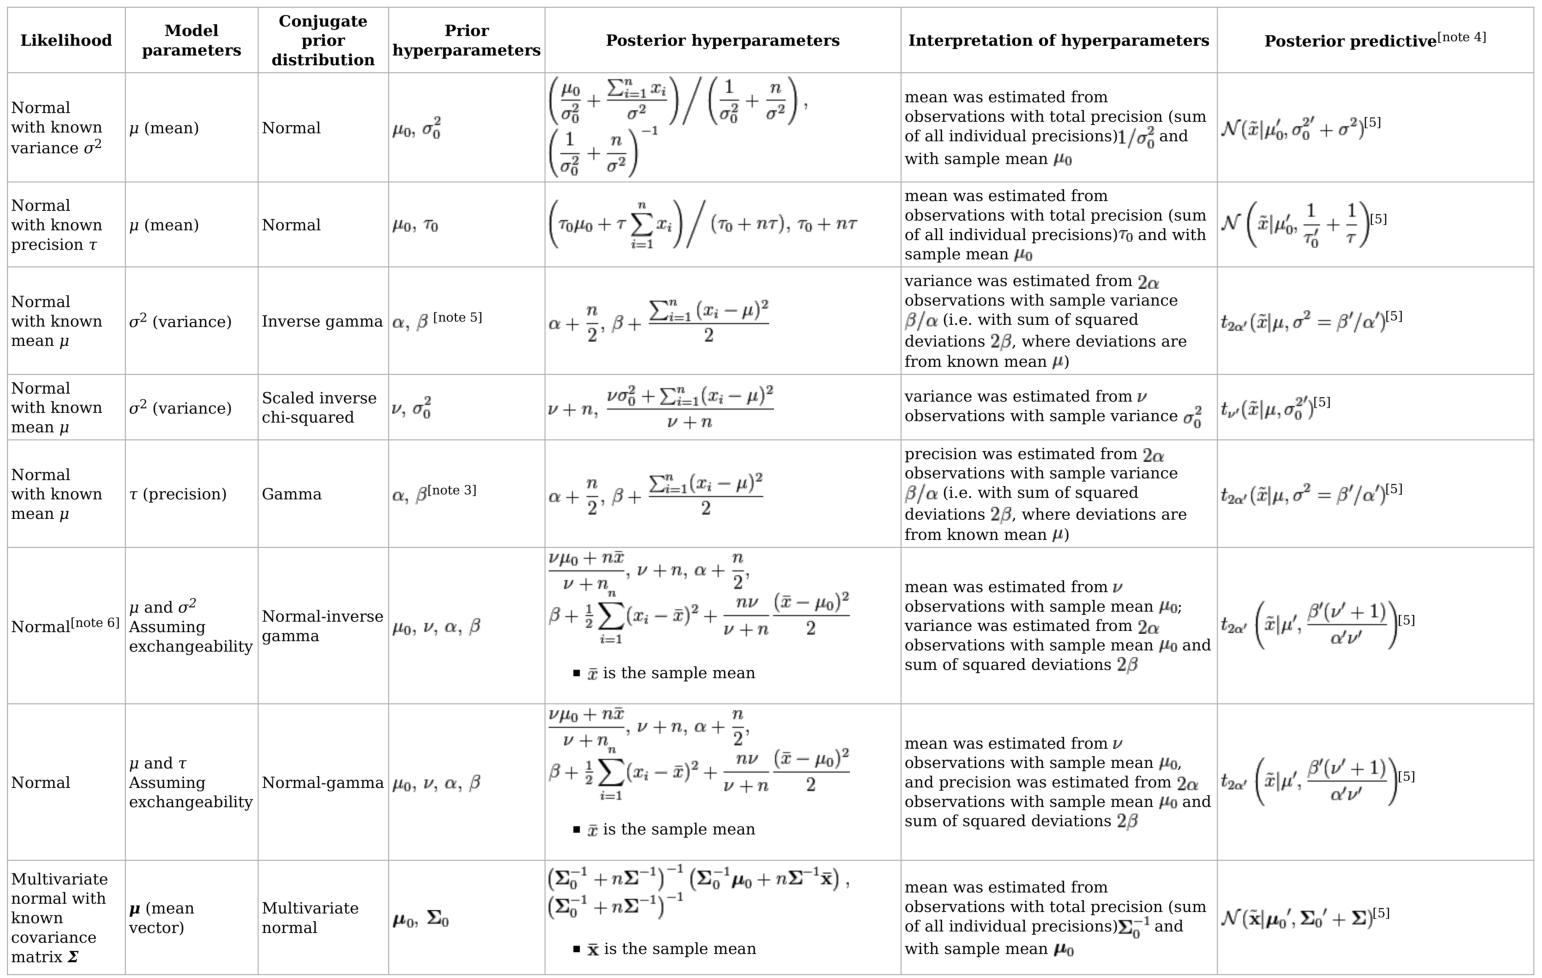
\includegraphics[width=1\textwidth]{../figs/WikipediaConjugatePrior-Continuous}

  \footnotesize{\url{en.wikipedia.org/wiki/Conjugate_prior}}
}

%====================================================================
\subsection{Monte Carlo integration}
\frame{\frametitle{Outline} \tableofcontents[currentsubsection]}
%====================================================================
\frame{ \frametitle{Computing integrals}

  \paragraph{General case:} $p(\thetabf \gv \Ybf)$ has no close form
  
  \bigskip 
  \paragraph{Goal:} compute
  $$
  \Esp(f(\thetabf) \gv \Ybf) 
  = \int f(\thetabf) p(\thetabf \gv \Ybf) \d \thetabf
  = \left. \int f(\thetabf) \pi(\thetabf) \; \ell(\Ybf \gv \thetabf) \d \thetabf \right/ p(\Ybf) 
  $$
  where
  $$
  p(\Ybf) = \int \pi(\thetabf) \; \ell(\Ybf \gv \thetabf) \d \thetabf 
  $$
  
  \bigskip \bigskip \pause
  We need to evaluate integrals of the form
  $$
  \int [\cdots] \; \emphase{\pi(\thetabf) \; \ell(\Ybf \gv \thetabf)} \d \thetabf 
  $$
}

%====================================================================
\frame{ \frametitle{Monte Carlo}

  \paragraph{Principle.} To evaluate
  $$
  \Esp_q[f(\thetabf)] = \int f(\thetabf) \emphase{q(\thetabf)} \d \thetabf
  $$
  \begin{enumerate}
   \item \pause sample 
   $$
   (\thetabf^1, \dots, \thetabf^M) \text{ iid } \sim q
   $$
   \item \pause compute
   $$
   \widehat{\Esp}_q[f(\thetabf)] = \frac1M \sum_m f(\thetabf^m)
   $$
  \end{enumerate}
  \pause \ra unbiased estimate of $\Esp_q[f(\thetabf)]$ with variance $\propto 1/ M$. \appref{app:MCillustration}
  
  \bigskip \bigskip \pause
  \paragraph{In practice:} 
  \begin{itemize}
   \item Works fine to evaluate $\Esp[f(\thetabf)]$, taking $q(\thetabf) = \pi(\thetabf)$
   $$
   \widehat{\Esp}_{\Ncal(0, 10)}\left[e^\theta\right] = \text{\tt mean(exp(rnorm(M, mean=0, sd=sqrt(10))))}
   $$\pause
   \item Useless to evaluate $\Esp[f(\thetabf) | \Ybf]$ as we do not know how to sample from $q(\thetabf) = p(\thetabf \gv \Ybf)$
  \end{itemize}
}

%===================================================================
\frame{ \frametitle{Importance Sampling (IS)}

  \paragraph{Main trick = weighting particles.} \pause To evaluate $\Esp[f(\thetabf)]$, write it as
  \begin{align*}
  \Esp_q[f(\thetabf)] 
  = \int f(\thetabf) q(\thetabf) \d \thetabf 
  = \int f(\thetabf) \frac{q(\thetabf)}{\emphase{q'(\thetabf)}} \emphase{q'(\thetabf)} \d \thetabf 
  \end{align*}
  for some \emphase{proposal} $q' \gg q$, from which you {\sl know how to sample}, then
  \begin{enumerate}
   \item \pause sample
   $$
   (\thetabf^1, \dots, \thetabf^M) \text{ iid } \sim \emphase{q'}(\thetabf),
   $$
   \item \pause compute the weights
   $$
   W(\thetabf^m) = q(\thetabf^m) / q'(\thetabf^m), 
   $$
   \item \pause and compute
   $$
   \widehat{\Esp}[f(\thetabf)] = \frac1M \sum_m W(\thetabf^m) f(\thetabf^m)
   $$
  \end{enumerate}
  \pause \ra unbiased estimate of $\Esp[f(\thetabf)]$ with variance $\propto \sum_m W(\theta^m)^2 / M$.

}  

%===================================================================
\frame{ \frametitle{Importance Sampling (a picture)}

  \begin{tabular}{cc}
    \begin{tabular}{p{.3\textwidth}}
	 \onslide+<4>{
	   Efficiency of sampling:
	   $$
	   ESS = \overline{W}^2 / \overline{W^2}
	   $$

	   \bigskip
	   $q' = q$
	   $$
	   \Rightarrow \quad ESS = 1
	   $$
	   }
    \end{tabular}
    & 
%     \hspace{-.\textwidth}
    \begin{tabular}{p{.5\textwidth}}
	 \begin{overprint}
	 \onslide<1>
	 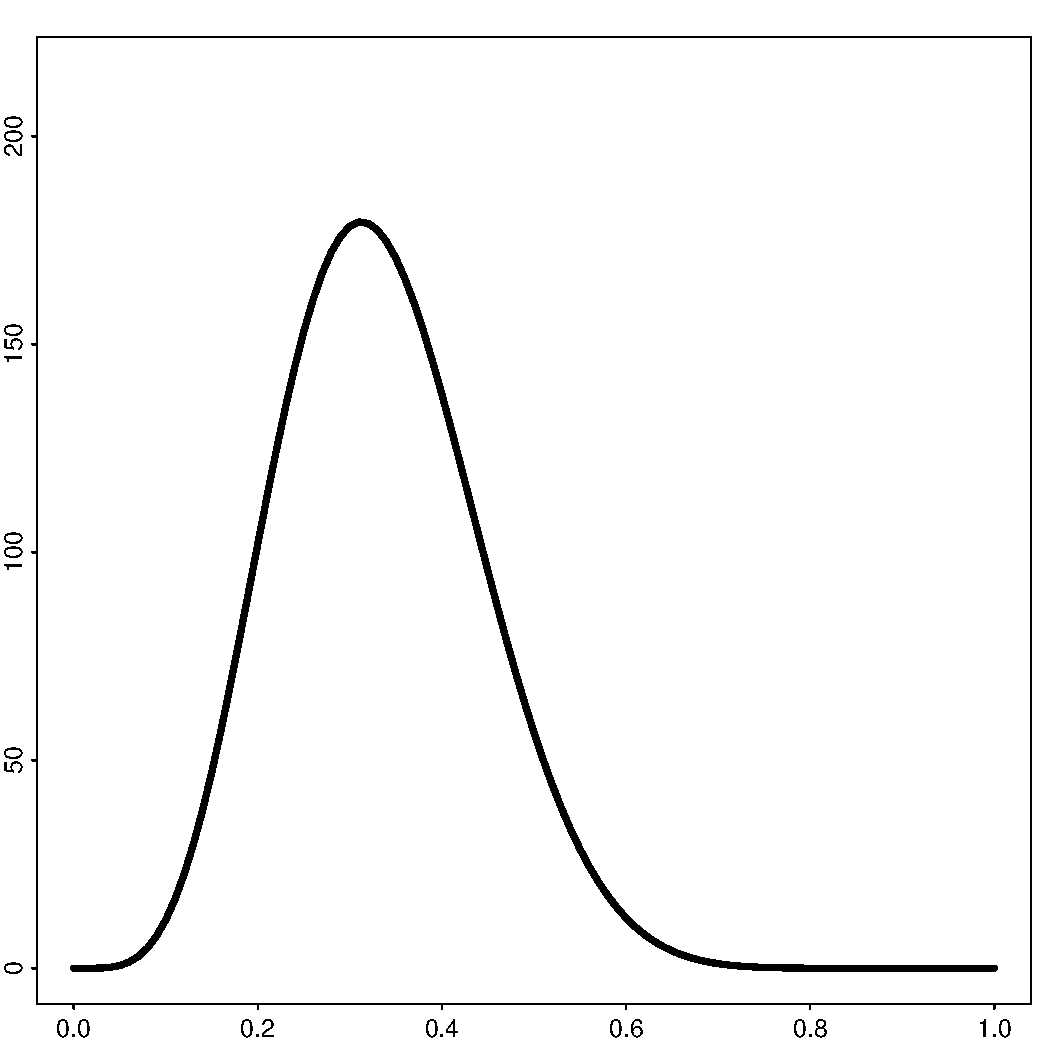
\includegraphics[height=.7\textheight]{../figs/ImportanceSampling-1}
	 \onslide<2>
	 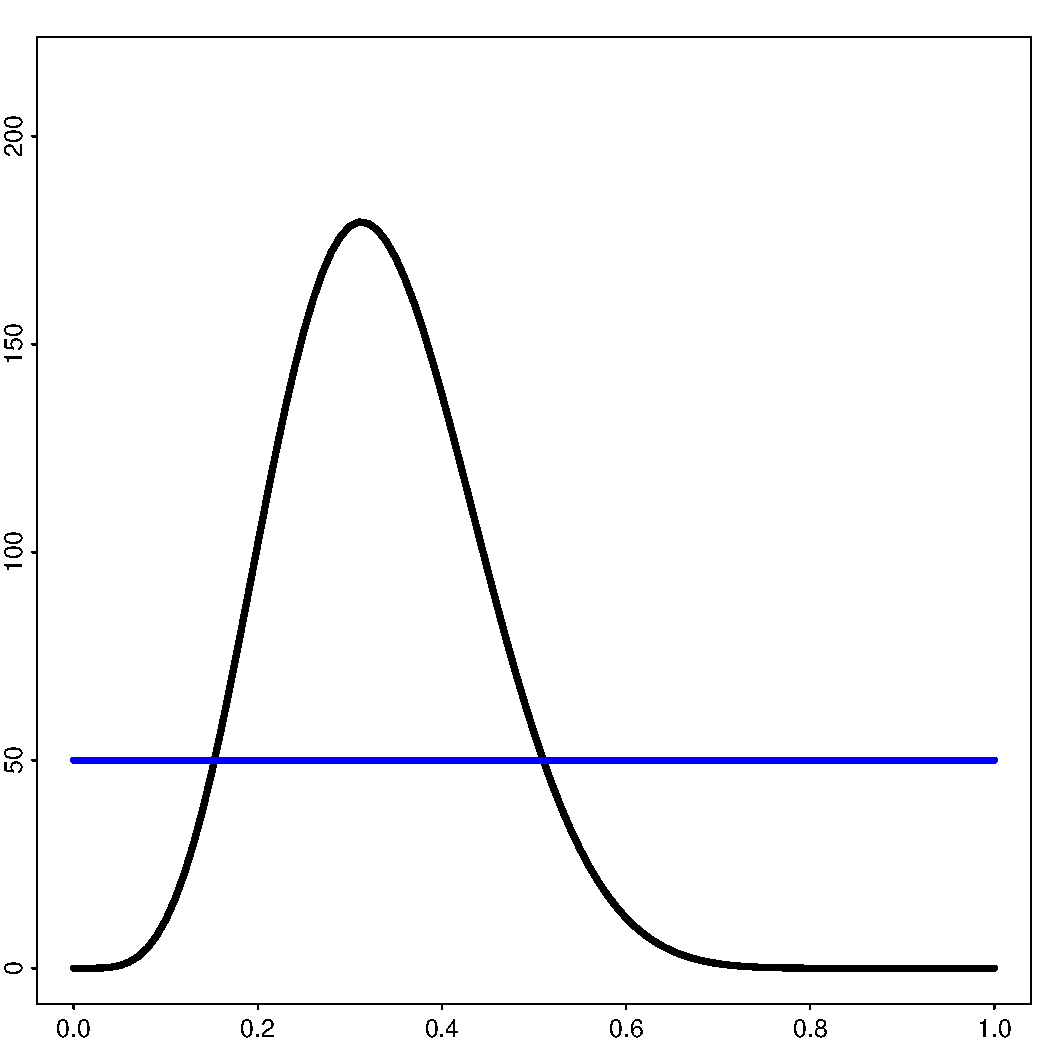
\includegraphics[height=.7\textheight]{../figs/ImportanceSampling-2}
	 \onslide<3>
	 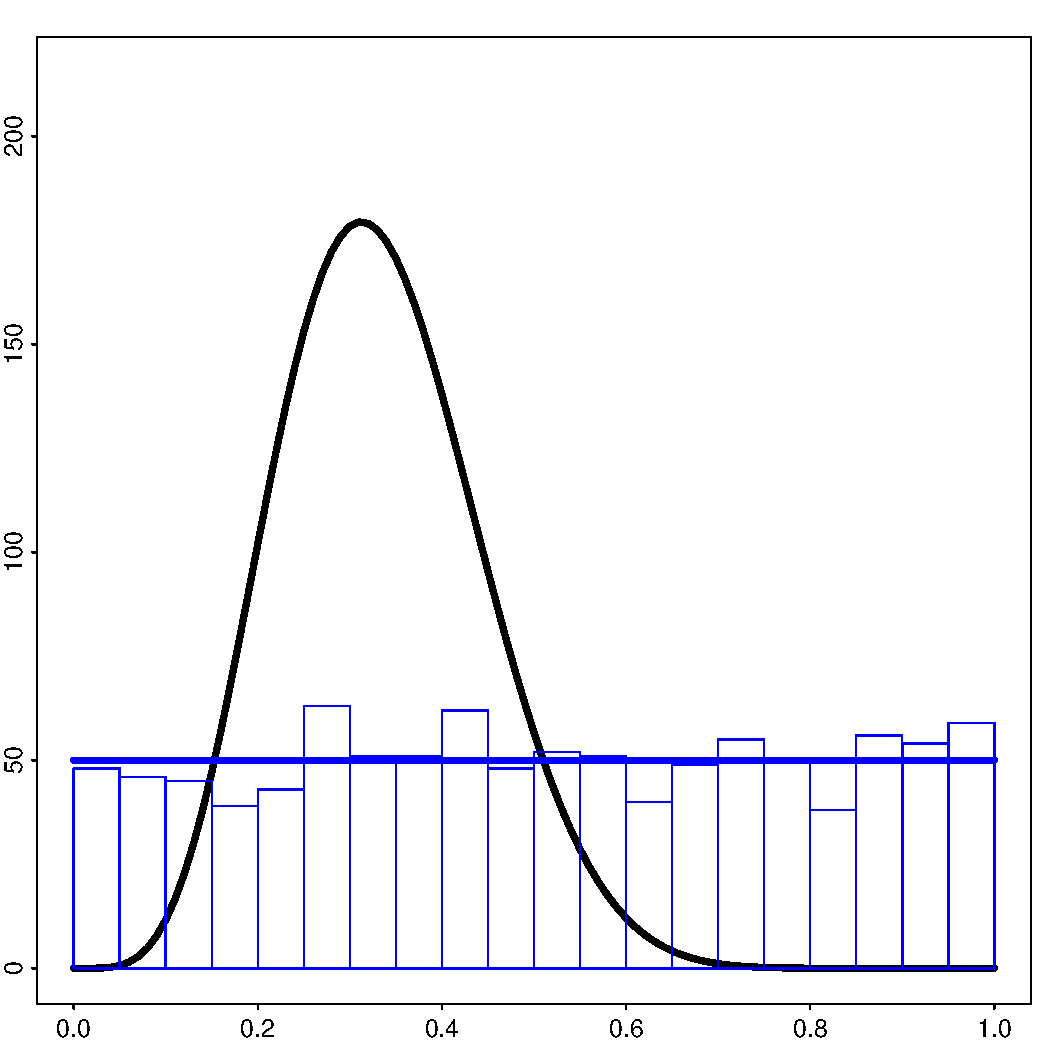
\includegraphics[height=.7\textheight]{../figs/ImportanceSampling-3}
	 \onslide<4>
	 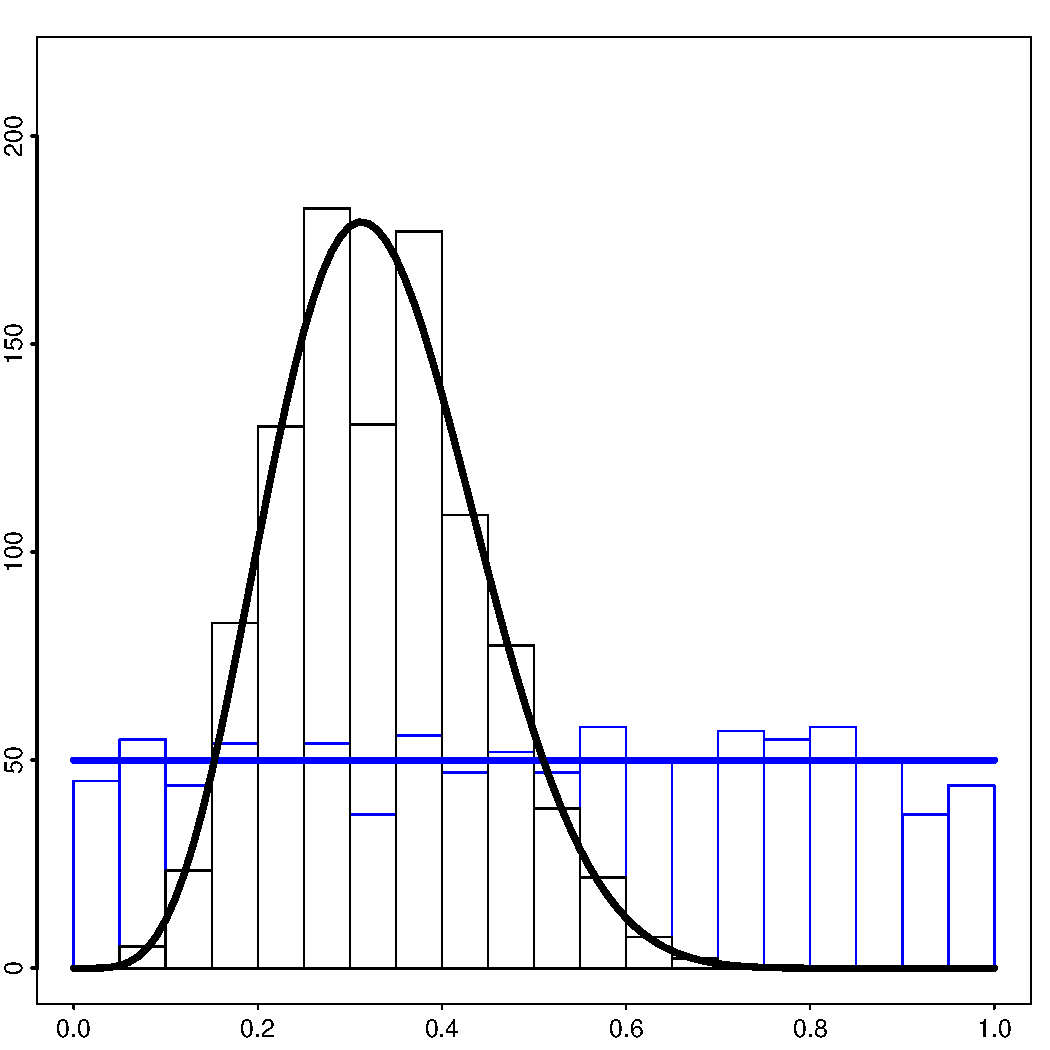
\includegraphics[height=.7\textheight]{../figs/ImportanceSampling-4}
	 \end{overprint}
    \end{tabular}
  \end{tabular}

}  


%===================================================================
\frame{ \frametitle{Importance Sampling: Importance of the proposal}

%   \begin{center}
%   \begin{tabular}{cc}
%     \begin{tabular}{c}
%     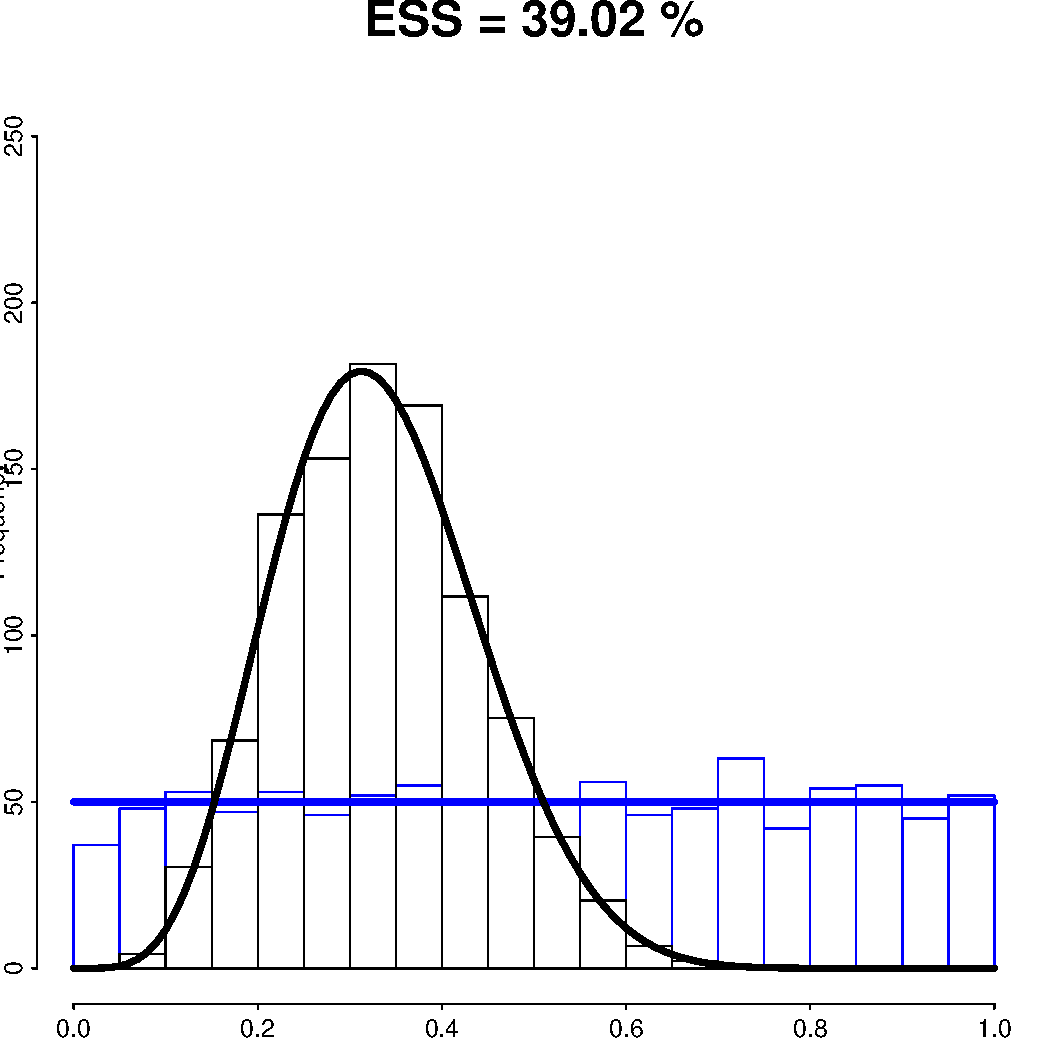
\includegraphics[height=.4\textheight]{../figs/ImportanceSampling-Beta-a06-b012-a1-b1-seed4} 
%     \end{tabular}
%     & 
%     \begin{tabular}{c}
%     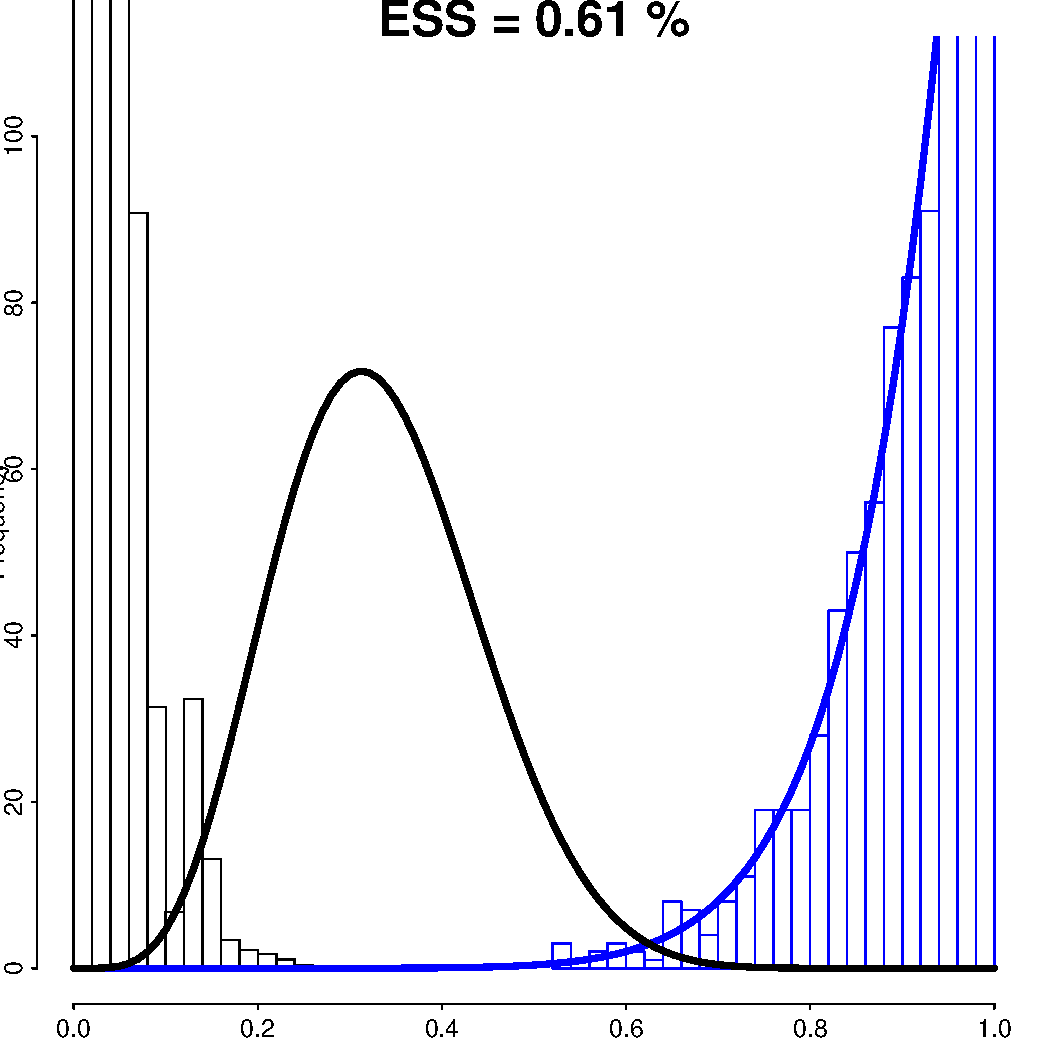
\includegraphics[height=.4\textheight]{../figs/ImportanceSampling-Beta-a06-b012-a10-b1-seed4} 
%     \end{tabular}
%     \\ \\
%     \begin{tabular}{c}
%     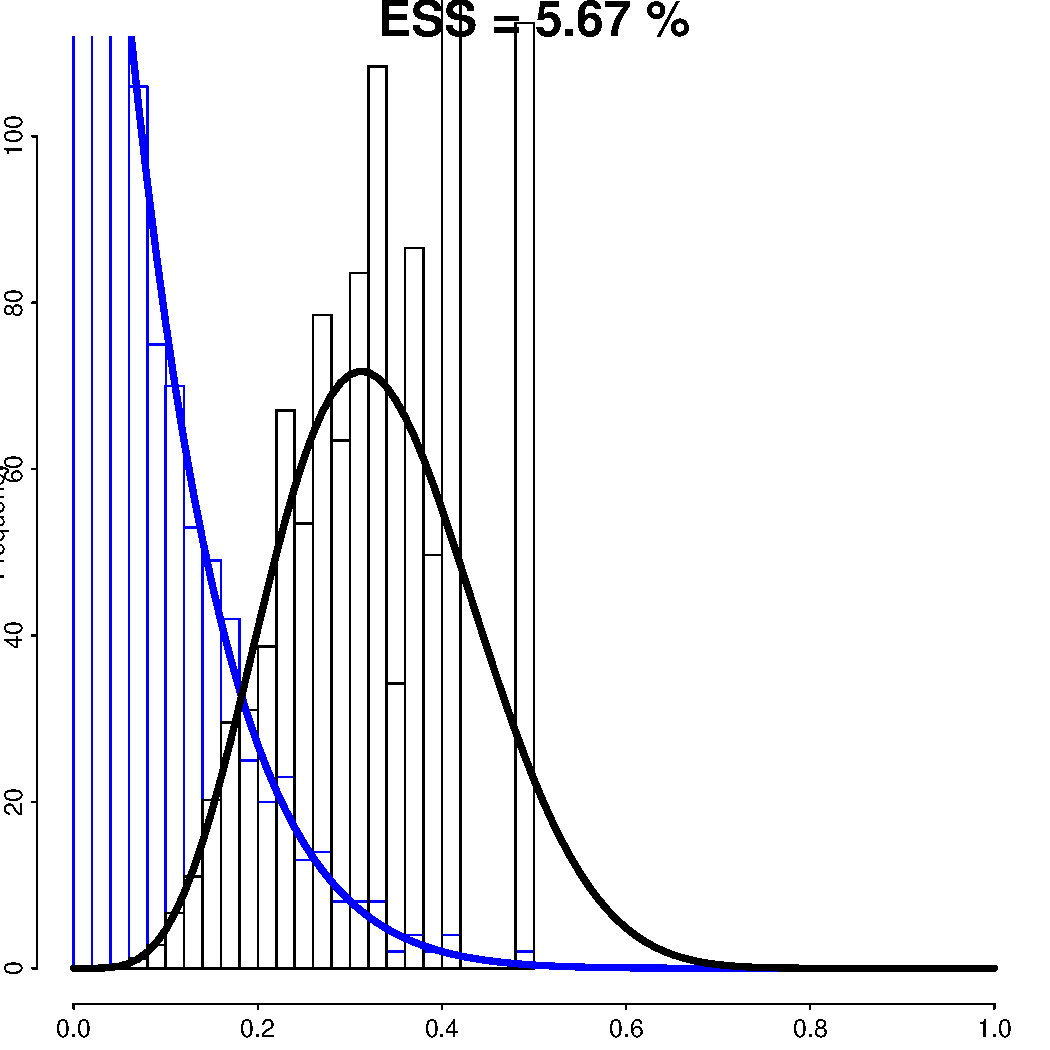
\includegraphics[height=.4\textheight]{../figs/ImportanceSampling-Beta-a06-b012-a1-b10-seed4} 
%     \end{tabular}
%     & 
%     \begin{tabular}{c}
%     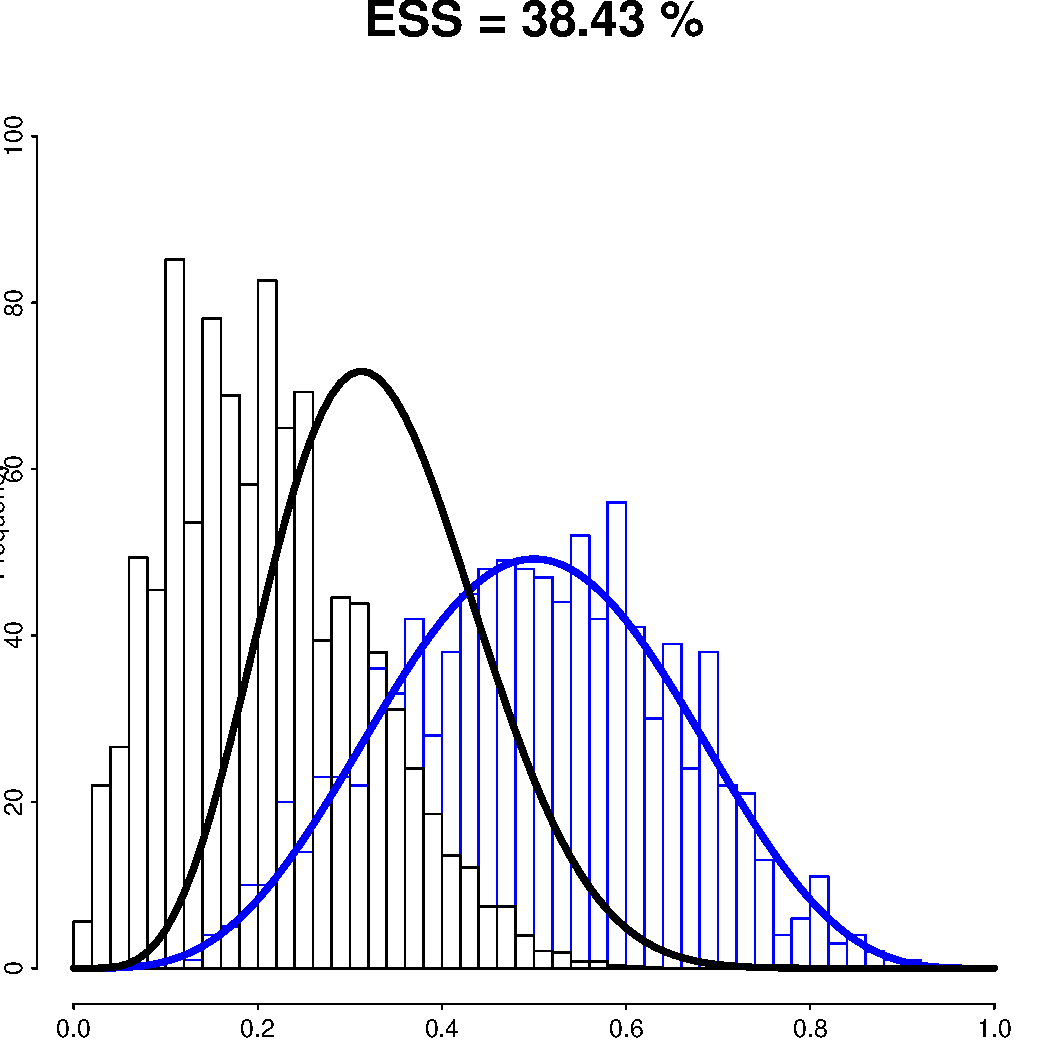
\includegraphics[height=.4\textheight]{../figs/ImportanceSampling-Beta-a06-b012-a5-b5-seed4} 
%     \end{tabular}
%   \end{tabular}
%   \end{center}
%  }  
% 
% %===================================================================
% \frame{ \frametitle{Importance of the proposal: another draw}

  \begin{center}
  \begin{tabular}{cc}
    \begin{tabular}{c}
    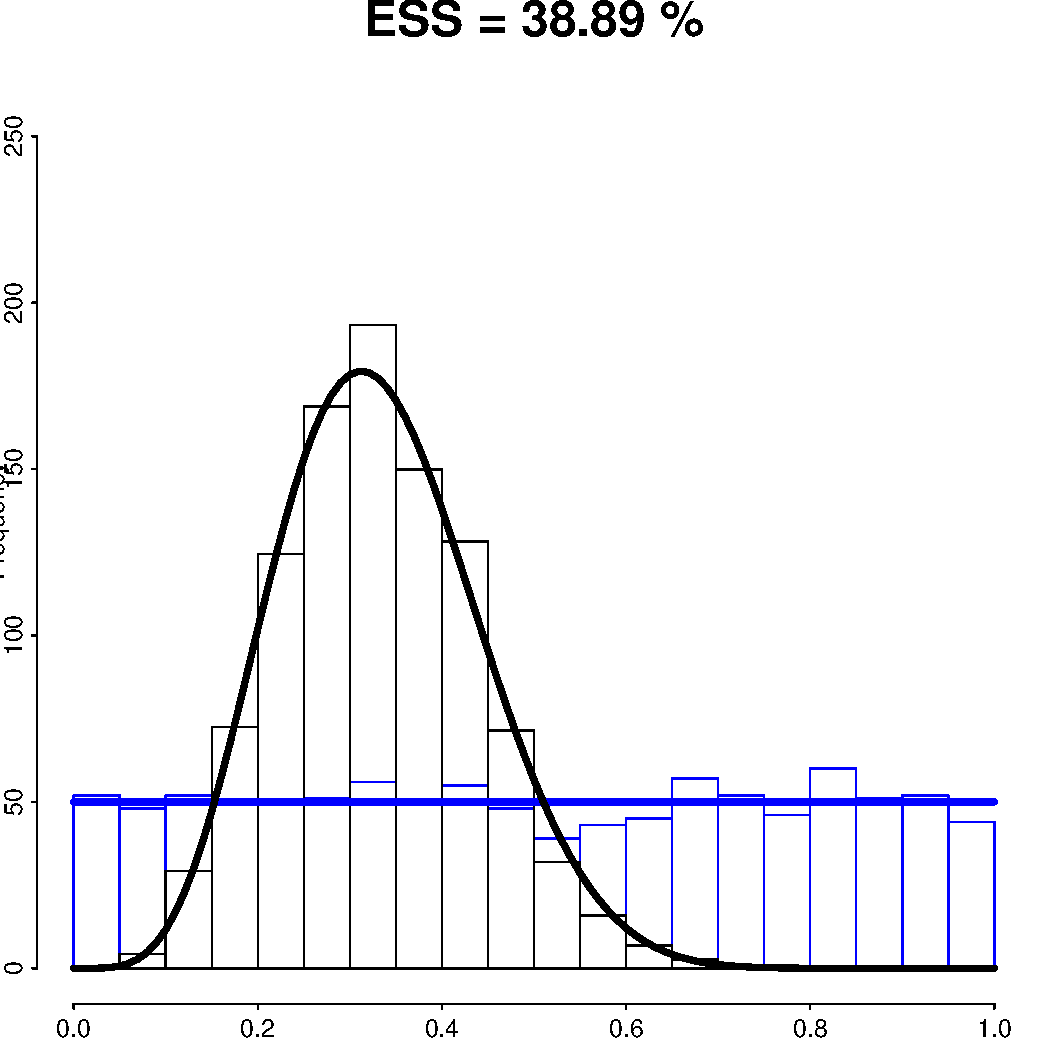
\includegraphics[height=.4\textheight]{../figs/ImportanceSampling-Beta-a06-b012-a1-b1-seed3} 
    \end{tabular}
    & 
    \begin{tabular}{c}
    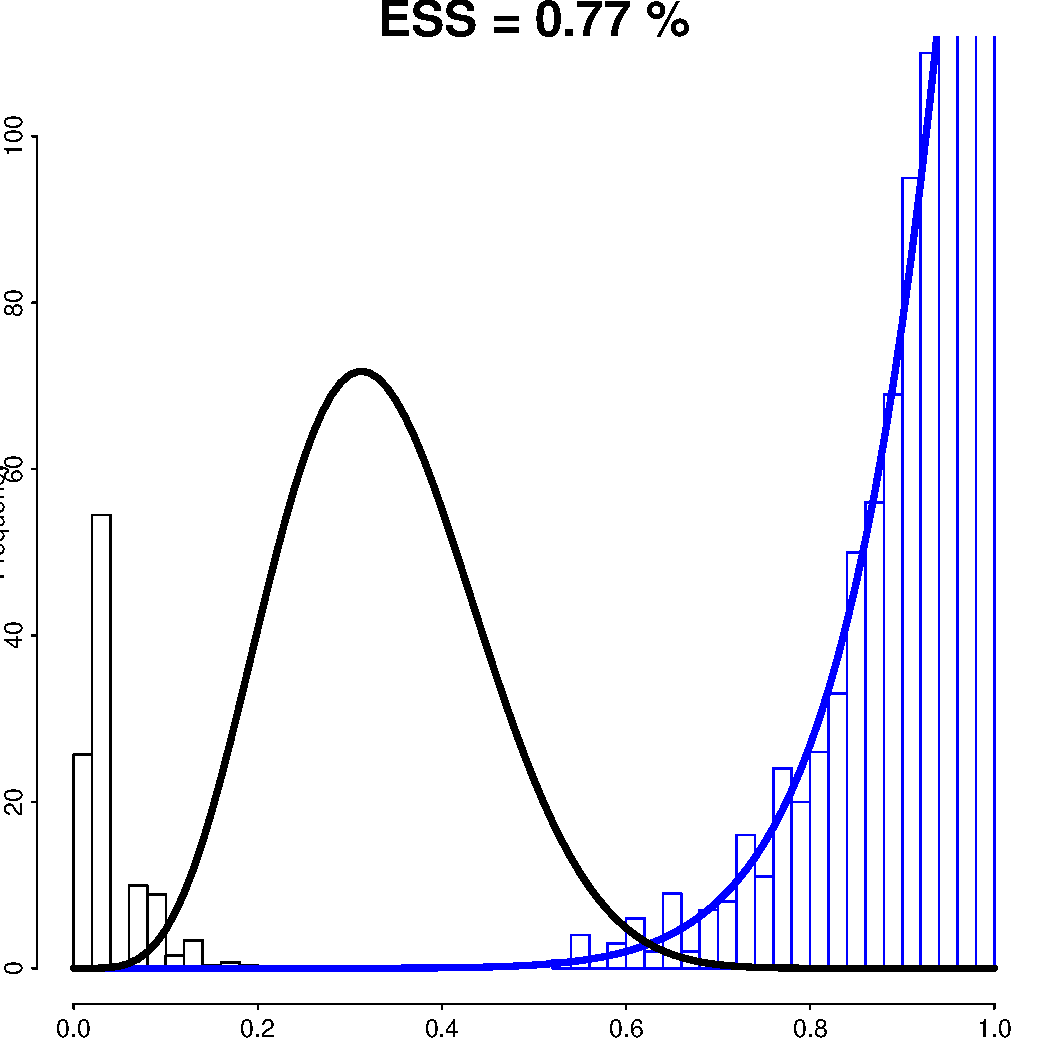
\includegraphics[height=.4\textheight]{../figs/ImportanceSampling-Beta-a06-b012-a10-b1-seed3} 
    \end{tabular}
    \\ \\
    \begin{tabular}{c}
    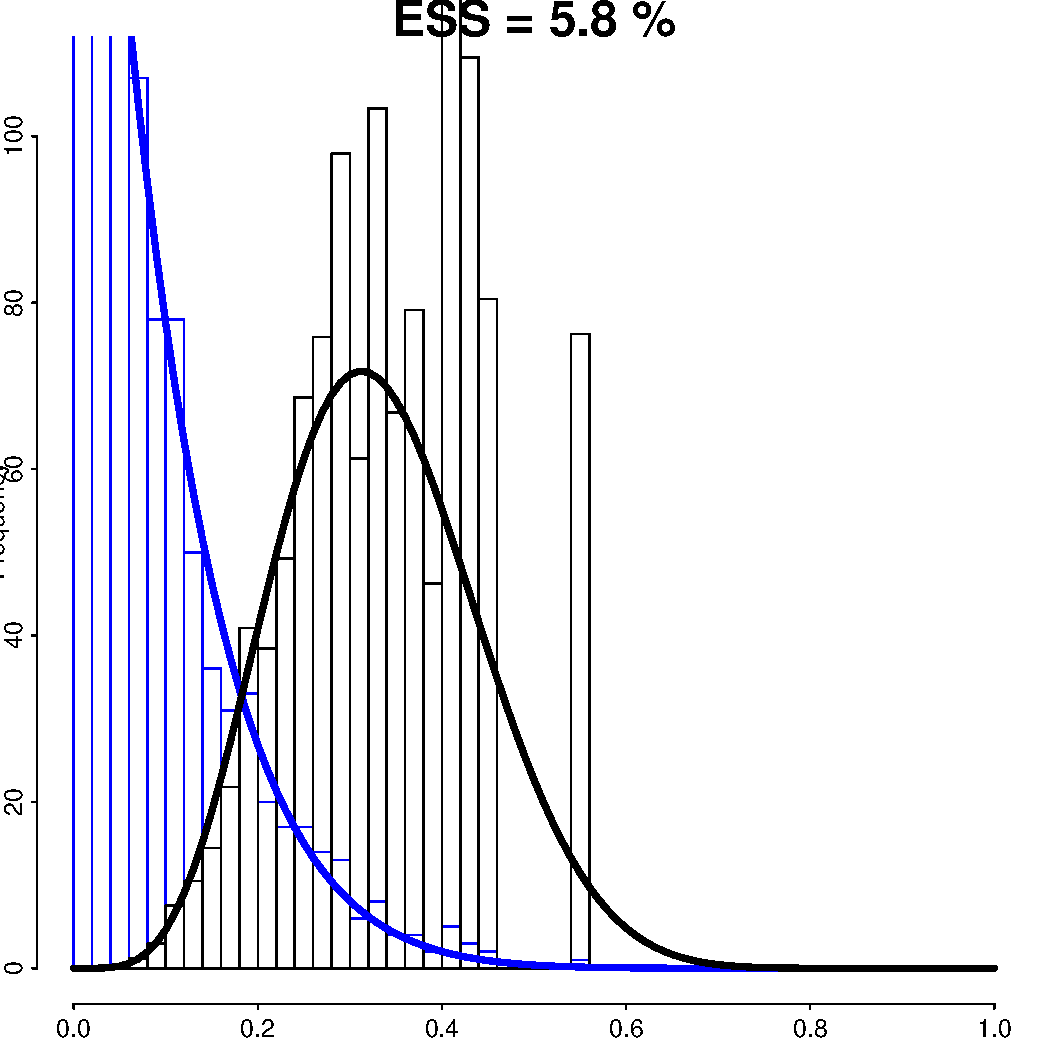
\includegraphics[height=.4\textheight]{../figs/ImportanceSampling-Beta-a06-b012-a1-b10-seed3} 
    \end{tabular}
    & 
    \begin{tabular}{c}
    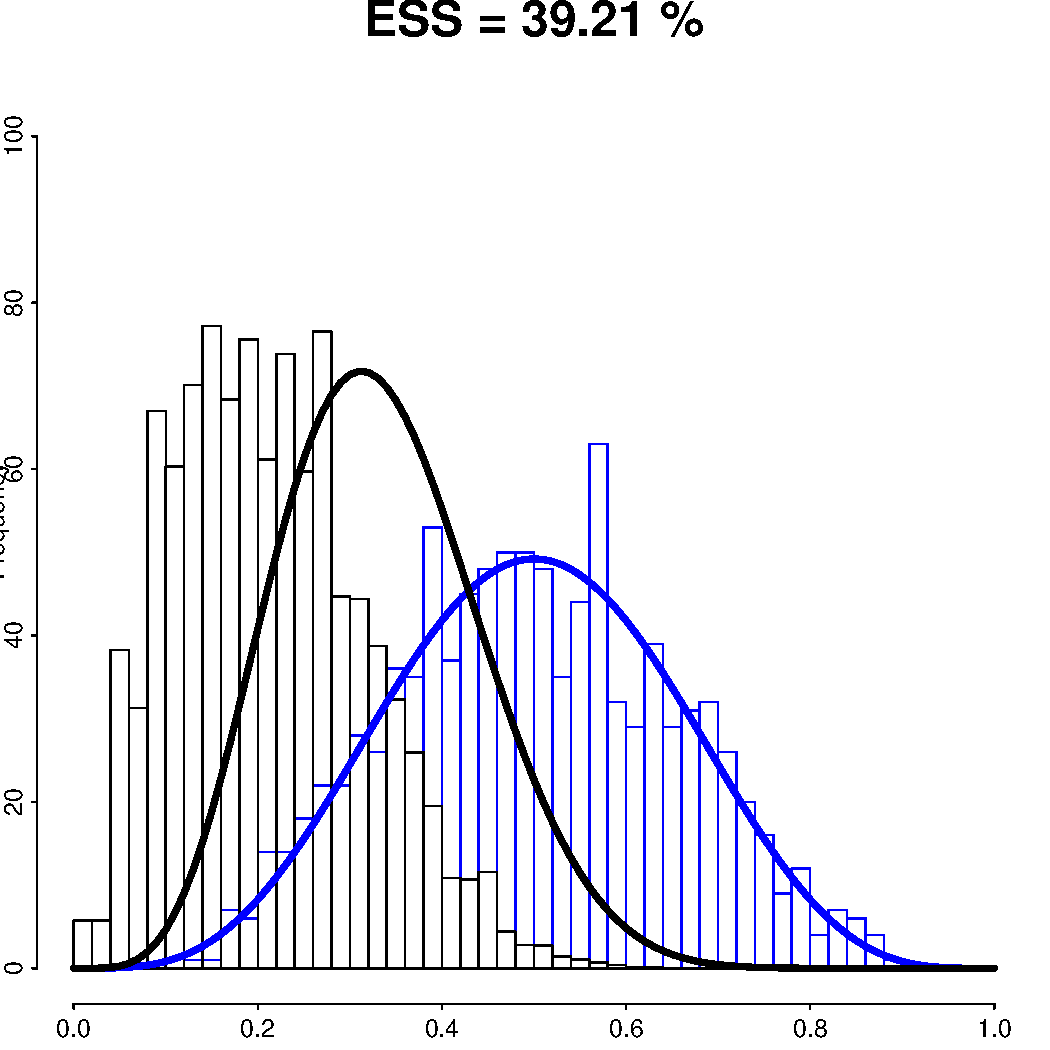
\includegraphics[height=.4\textheight]{../figs/ImportanceSampling-Beta-a06-b012-a5-b5-seed3} 
    \end{tabular}
  \end{tabular}
  \end{center}
 }  

%===================================================================
\frame{ \frametitle{Importance of the proposal: another draw}

  \begin{center}
  \begin{tabular}{cc}
    \begin{tabular}{c}
    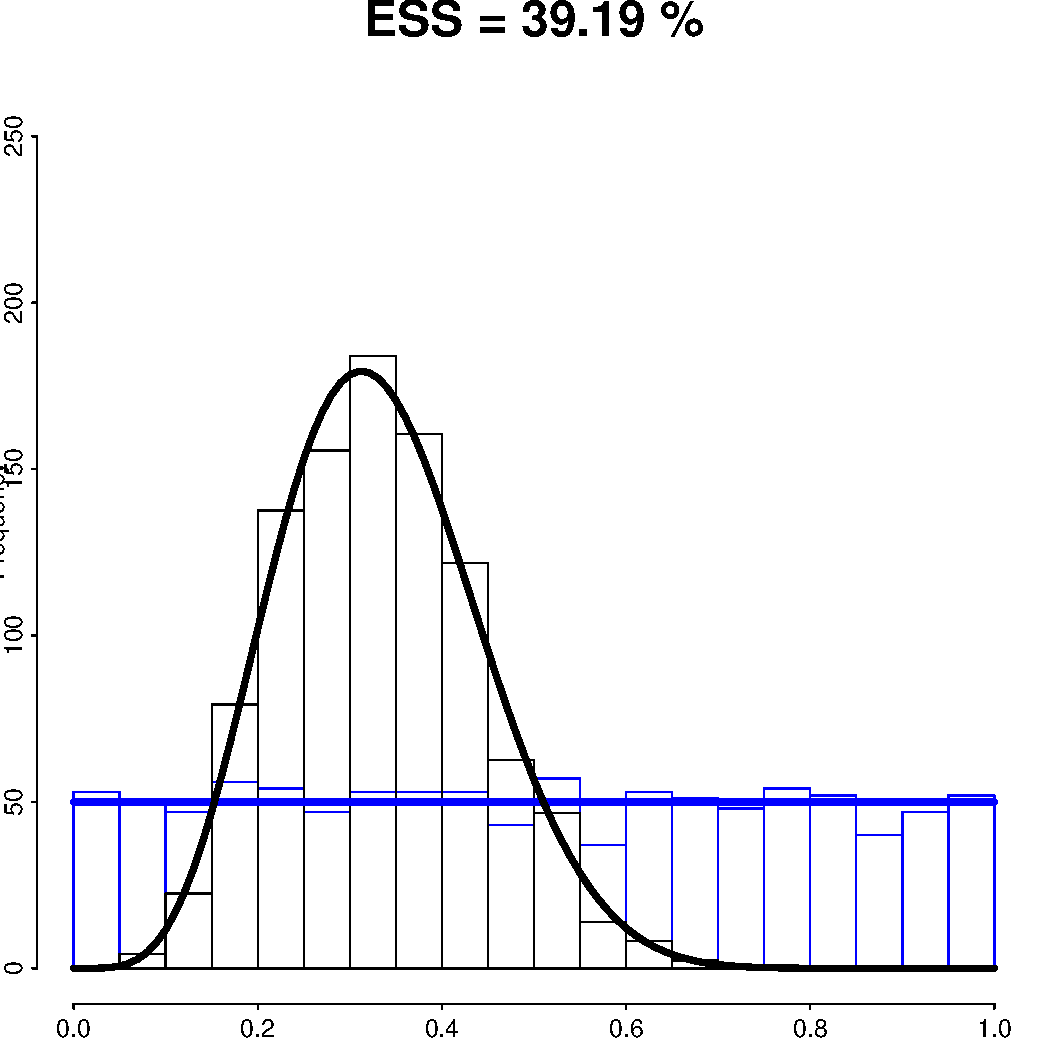
\includegraphics[height=.4\textheight]{../figs/ImportanceSampling-Beta-a06-b012-a1-b1-seed5} 
    \end{tabular}
    & 
    \begin{tabular}{c}
    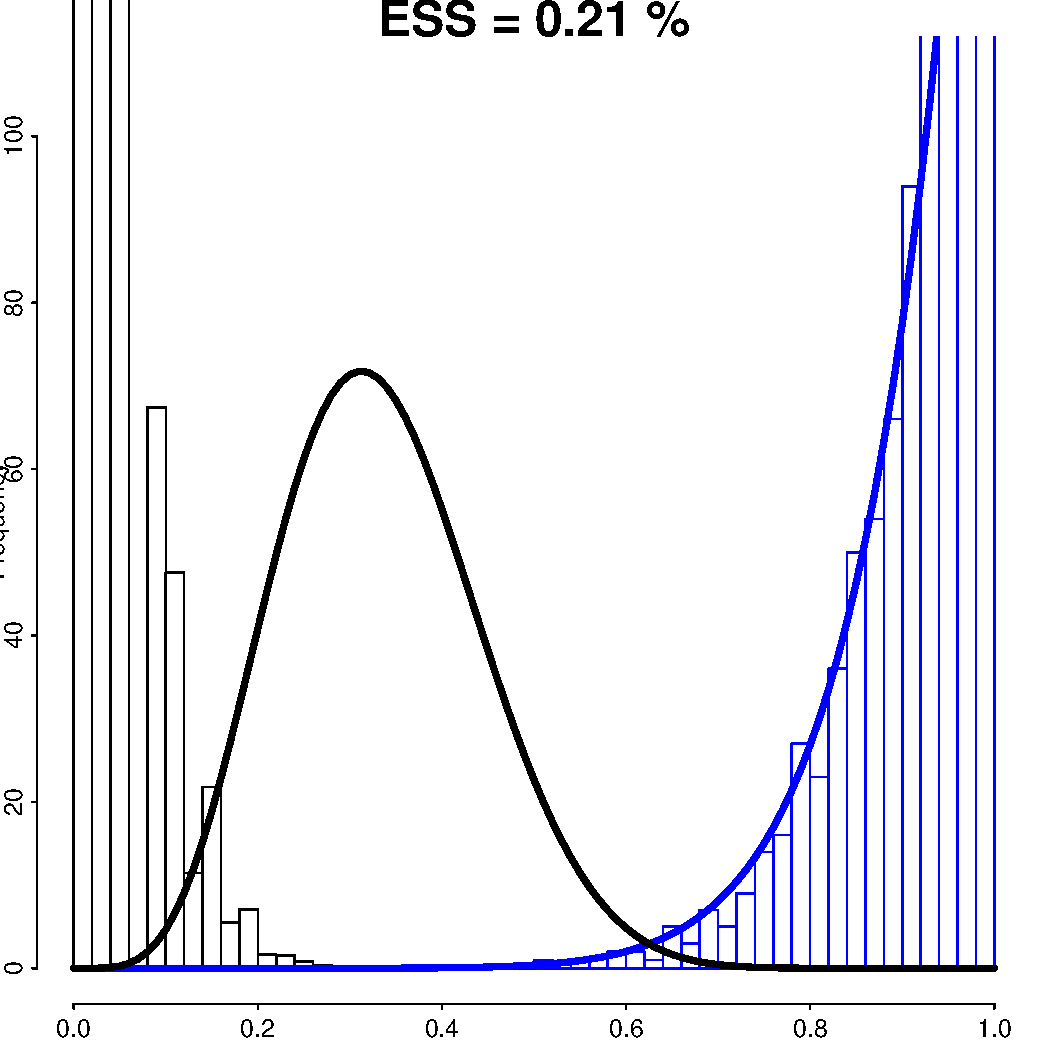
\includegraphics[height=.4\textheight]{../figs/ImportanceSampling-Beta-a06-b012-a10-b1-seed5} 
    \end{tabular}
    \\ \\
    \begin{tabular}{c}
    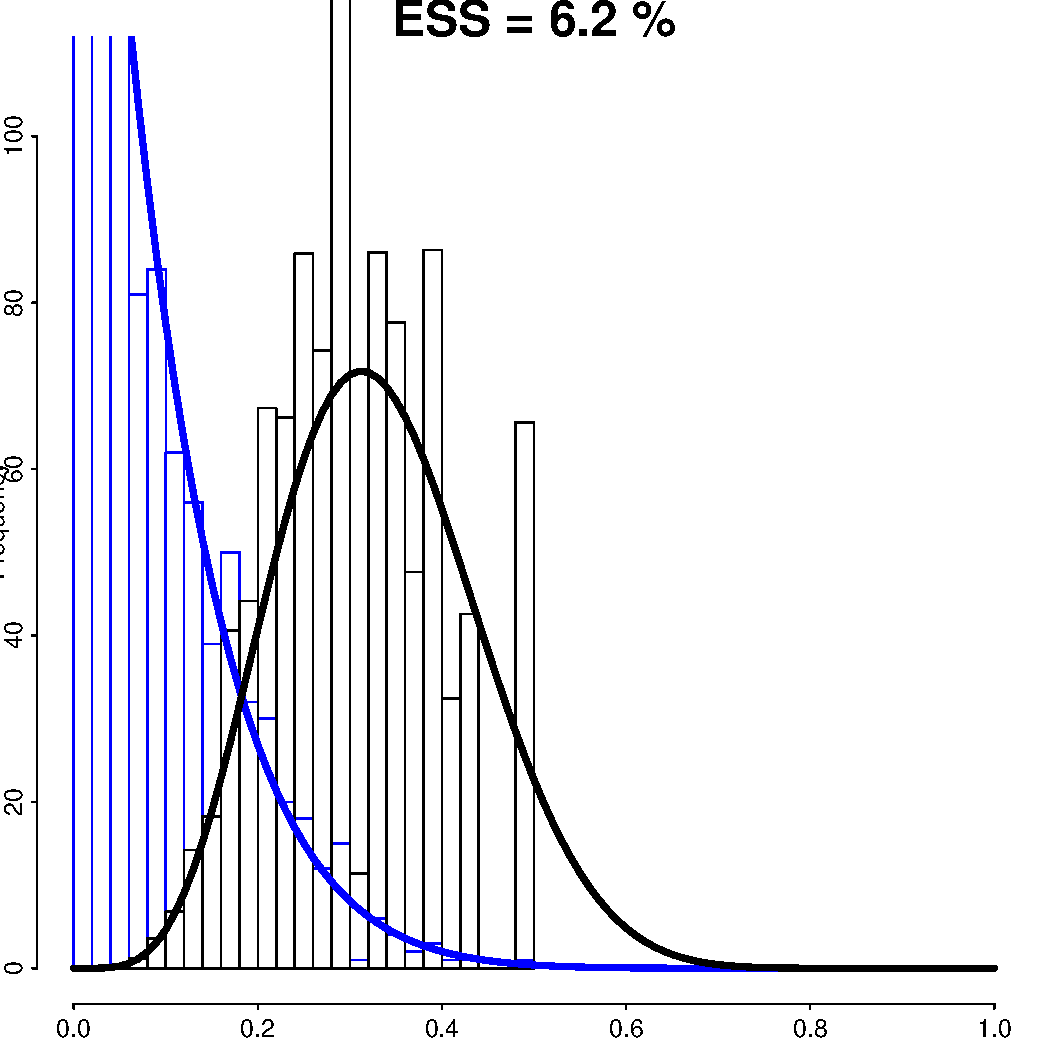
\includegraphics[height=.4\textheight]{../figs/ImportanceSampling-Beta-a06-b012-a1-b10-seed5} 
    \end{tabular}
    & 
    \begin{tabular}{c}
    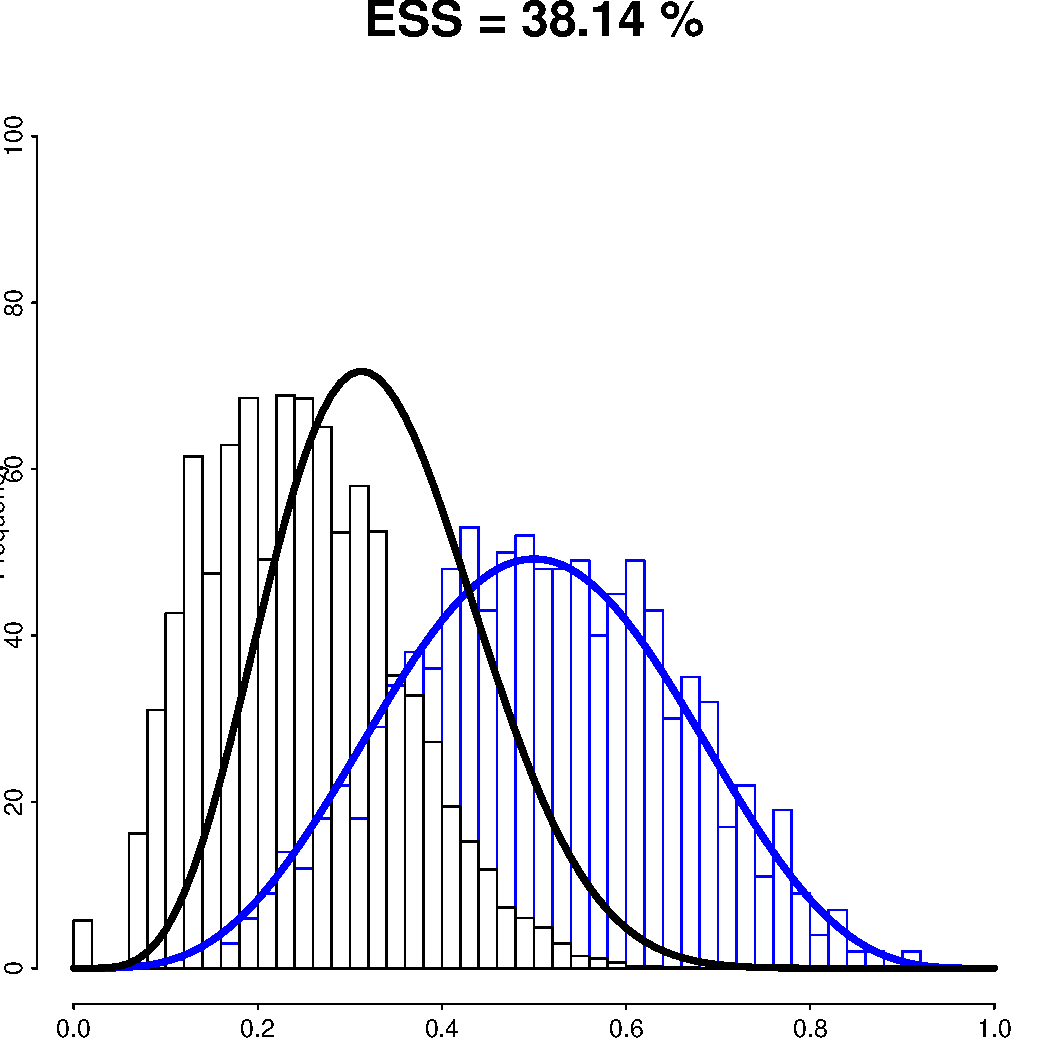
\includegraphics[height=.4\textheight]{../figs/ImportanceSampling-Beta-a06-b012-a5-b5-seed5} 
    \end{tabular}
  \end{tabular}
  \end{center}
 }  

% %===================================================================
% \frame{ \frametitle{Importance of the proposal: another draw}
% 
%   \begin{center}
%   \begin{tabular}{cc}
%     \begin{tabular}{c}
%     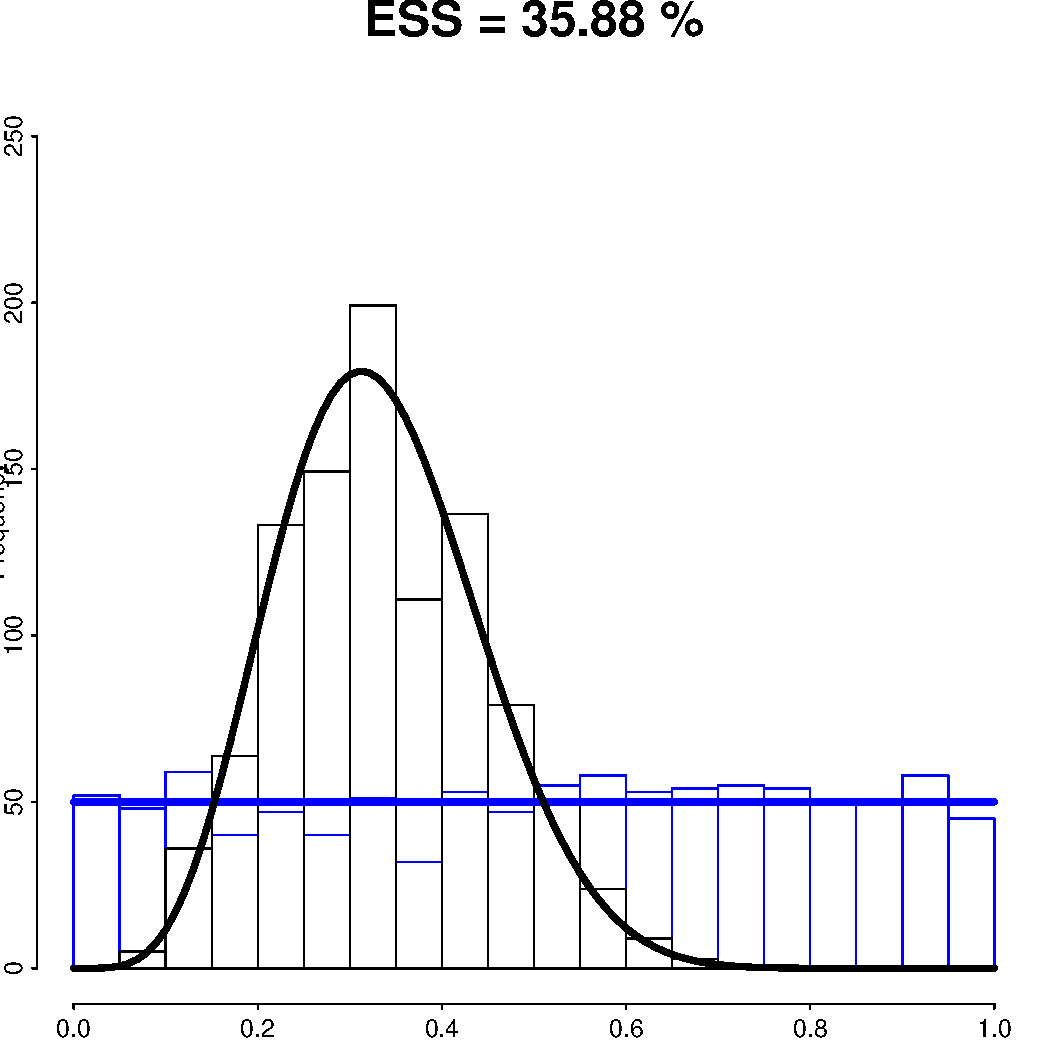
\includegraphics[height=.4\textheight]{../figs/ImportanceSampling-Beta-a06-b012-a1-b1-seed6} 
%     \end{tabular}
%     & 
%     \begin{tabular}{c}
%     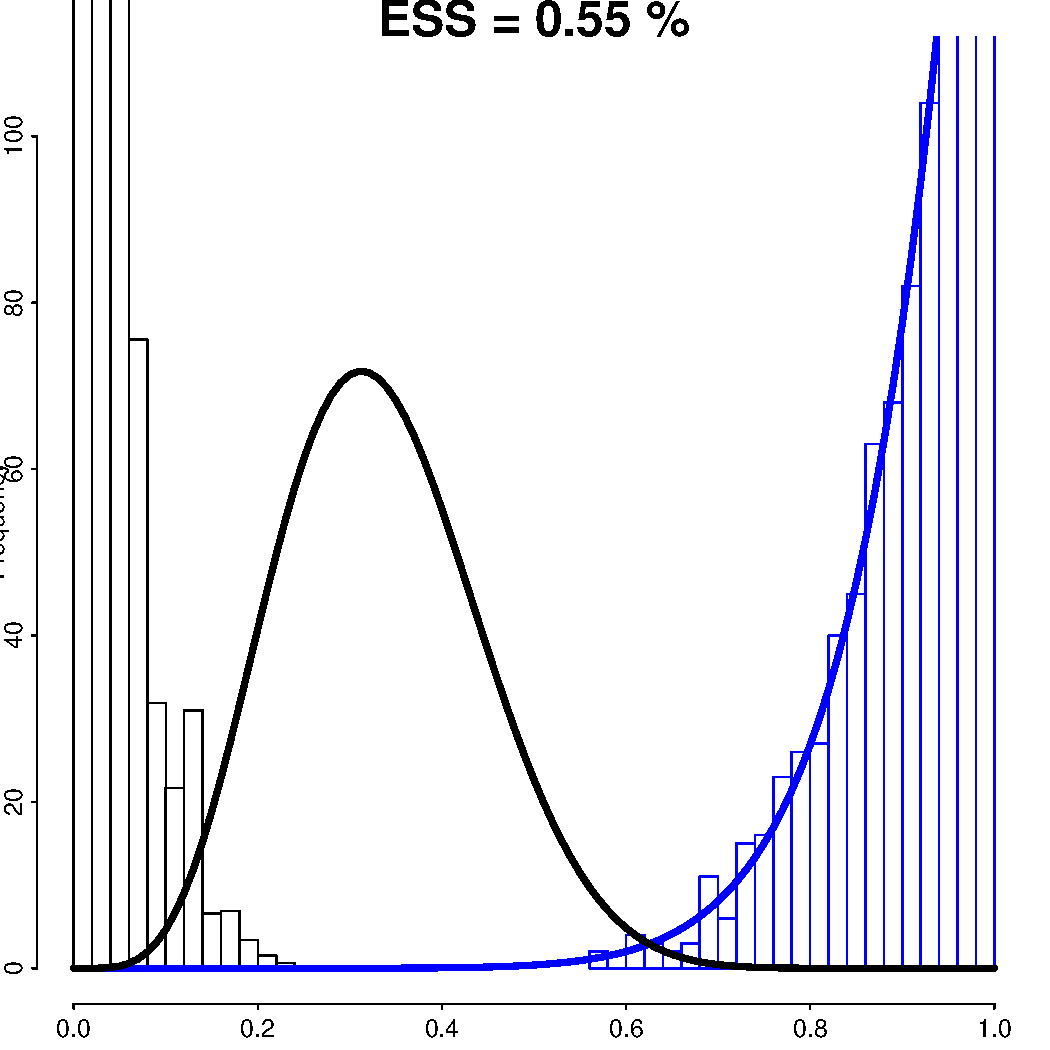
\includegraphics[height=.4\textheight]{../figs/ImportanceSampling-Beta-a06-b012-a10-b1-seed6} 
%     \end{tabular}
%     \\ \\
%     \begin{tabular}{c}
%     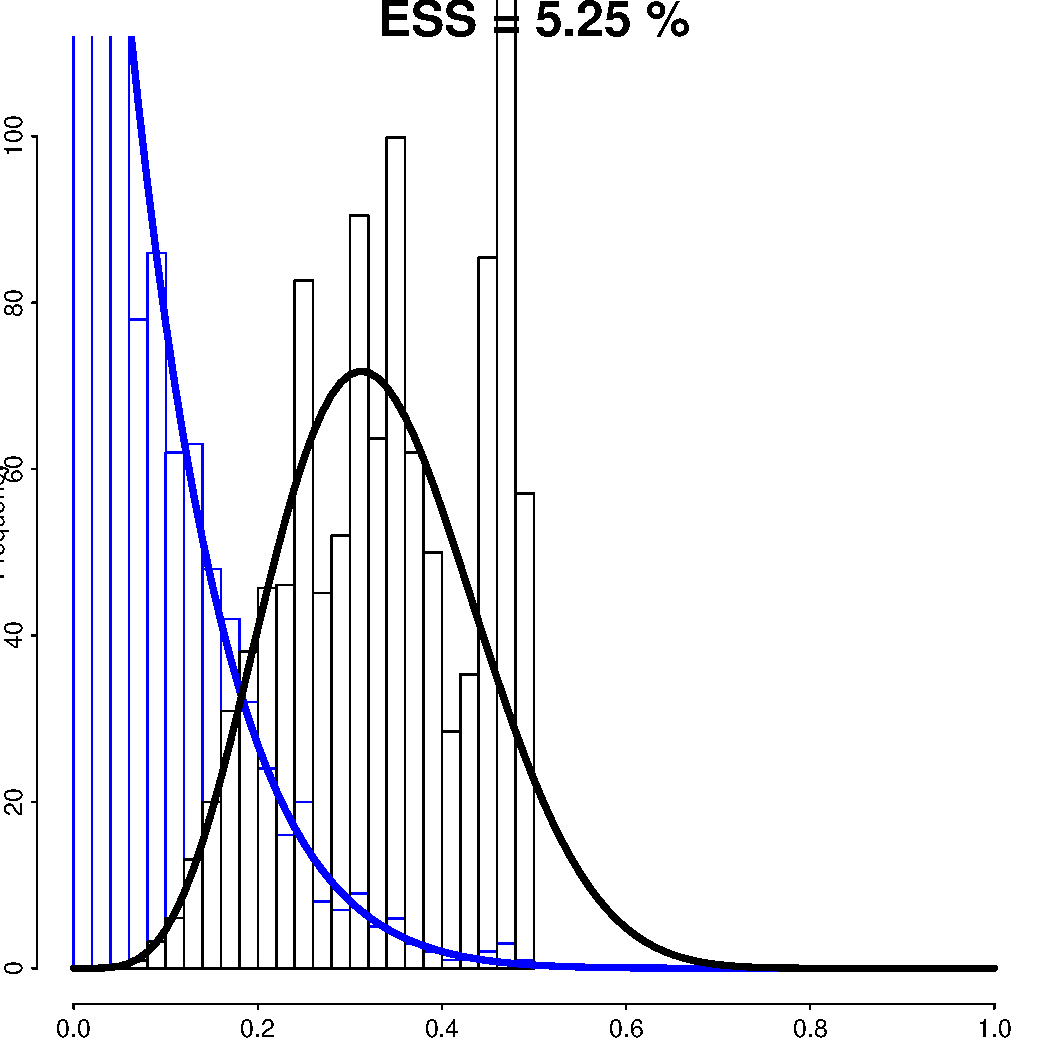
\includegraphics[height=.4\textheight]{../figs/ImportanceSampling-Beta-a06-b012-a1-b10-seed6} 
%     \end{tabular}
%     & 
%     \begin{tabular}{c}
%     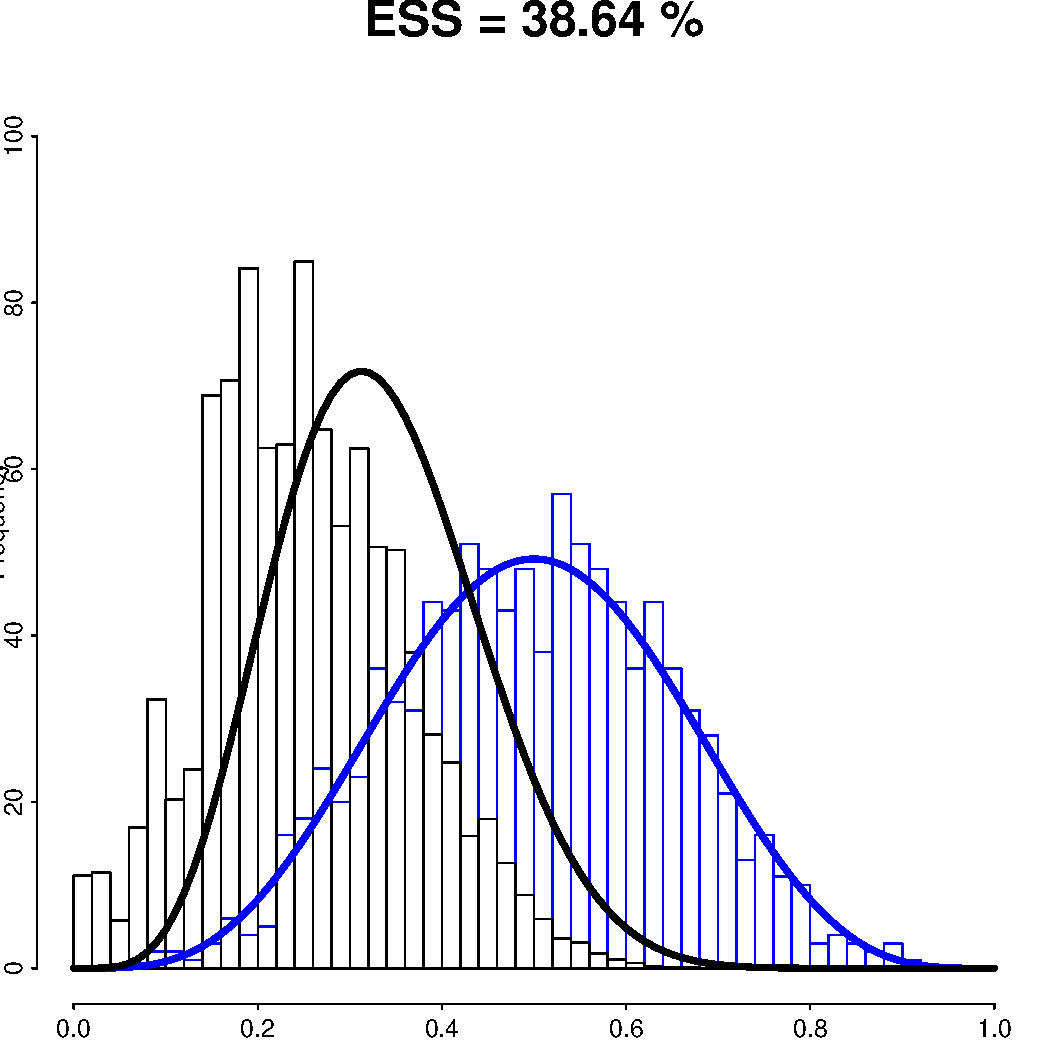
\includegraphics[height=.4\textheight]{../figs/ImportanceSampling-Beta-a06-b012-a5-b5-seed6} 
%     \end{tabular}
%   \end{tabular}
%   \end{center}
%  }  
% 
%===================================================================
\frame{ \frametitle{IS for posterior sampling}

  To evaluate $\Esp[f(\thetabf) | \Ybf]$, write it as
  \begin{align*}
    \Esp[f(\thetabf) \gv \Ybf] 
    = & \left. \int f(\thetabf) p(\thetabf, \Ybf) \d \thetabf \right/ p(\Ybf) 
    \; = \; \dots \\
%     = & \left. \int f(\thetabf) \pi(\thetabf) \ell(\Ybf \gv \thetabf) \d \thetabf \right/ \int \pi(\thetabf) \ell(\Ybf \gv \thetabf)  \d \thetabf \\
    = & \left. \int f(\thetabf) \frac{\pi(\thetabf) p(\thetabf \gv \Ybf)}{q(\thetabf)} q(\thetabf) \d \thetabf \right/ \int \frac{\pi(\thetabf) p(\thetabf \gv \Ybf)}{q(\thetabf)} q(\thetabf) \d \thetabf
  \end{align*}
  \begin{enumerate}
   \item sample
   $$
   (\thetabf^1, \dots, \thetabf^M) \text{ iid } \sim q
   $$
   \item compute the weights
   $$
   W(\thetabf^m) = \pi(\thetabf^m) p(\thetabf^m \gv \Ybf) \left/ q(\thetabf^m) \right.
   $$
   \item get
   $$
   \widehat{\Esp}[f(\thetabf) \gv \Ybf] = \sum_m W(\thetabf^m) f(\thetabf^m) \left/ \sum_m W(\thetabf^m)  \right.
   $$
   \ra slightly biased.
  \end{enumerate}
}

%===================================================================
\frame{ \frametitle{Good proposals}

  Choosing $q$ is critical

  \bigskip \pause
  \paragraph{Typical choices}
  \begin{itemize}
   \item Prior
   $$q(\thetabf) = \pi(\thetabf)$$
   \ra {far from the target $p(\thetabf \gv \Ybf)$: small $ESS$} \\ ~
   \item \pause MLE: 
   $$q(\thetabf) = \Ncal(\widehat{\thetabf}_{MLE}, \Var_\infty(\widehat{\thetabf}_{MLE}))$$  
   \ra {fine, as long as MLE is available} \\ ~
   \item \pause Variational Bayes, expectation propagation, ...: 
   $$
   q(\thetabf) = \arg\min_{q \in \Qcal} KL\left[q(\thetabf) \,||\, p(\thetabf \gv \Ybf\right]
   $$
   \ra fast and reasonably accurate
  \end{itemize}
}

%===================================================================
\frame{ \frametitle{Variational Bayes \& ML as a prior}

  $\textcolor{blue}{\boldsymbol{-}}:$ prior, $\textcolor{red}{\boldsymbol{-}}:$ VB, $\textcolor{green}{\boldsymbol{-}}:$ MLE, $\boldsymbol{-}:$ posterior 
  $$
  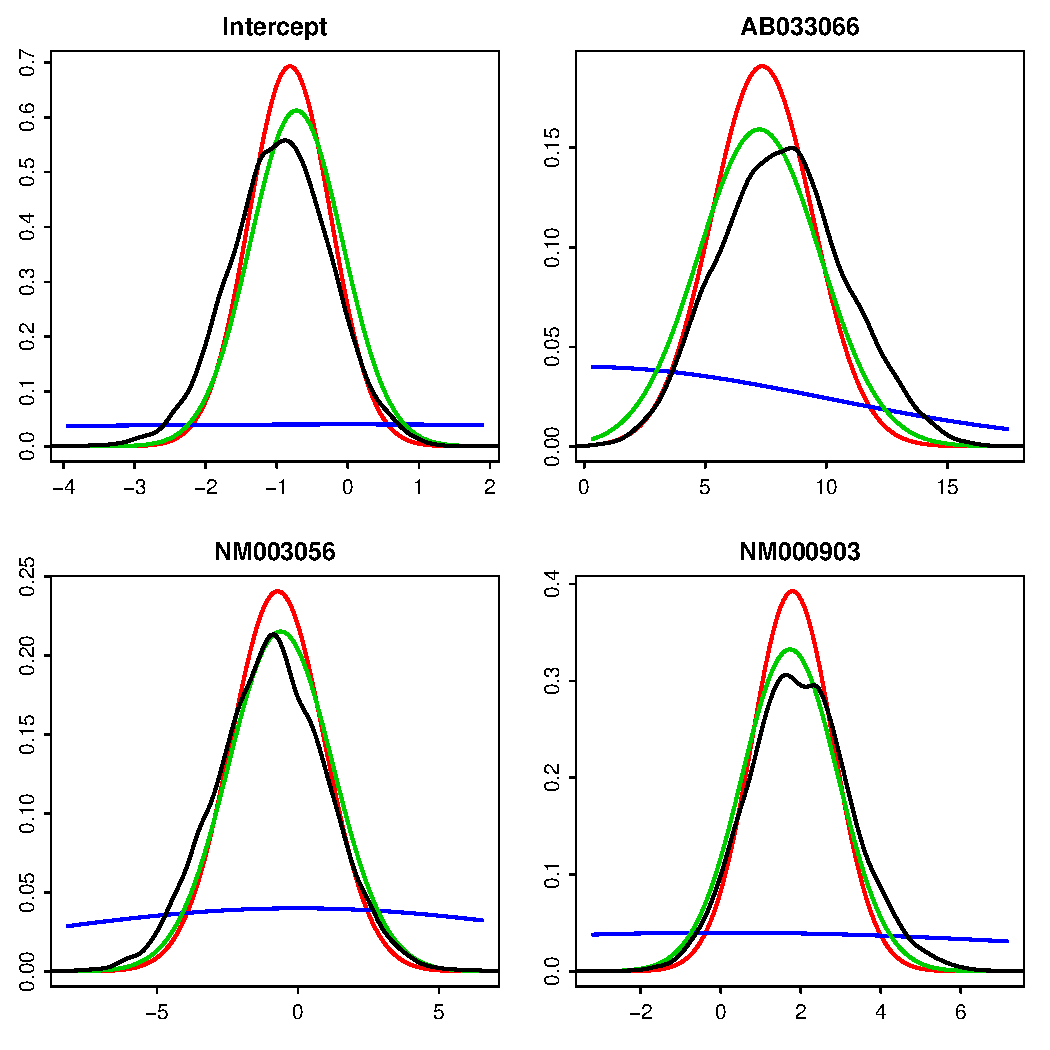
\includegraphics[width=.8\textwidth, height=.8\textheight]{\figfig/ISproposal-density}
  $$
}

%===================================================================
\frame{ \frametitle{Variational Bayes as a prior: joint distribution}

  $\textcolor{red}{\boldsymbol{-}}:$ VB, $\boldsymbol{-}:$ posterior 
  $$
  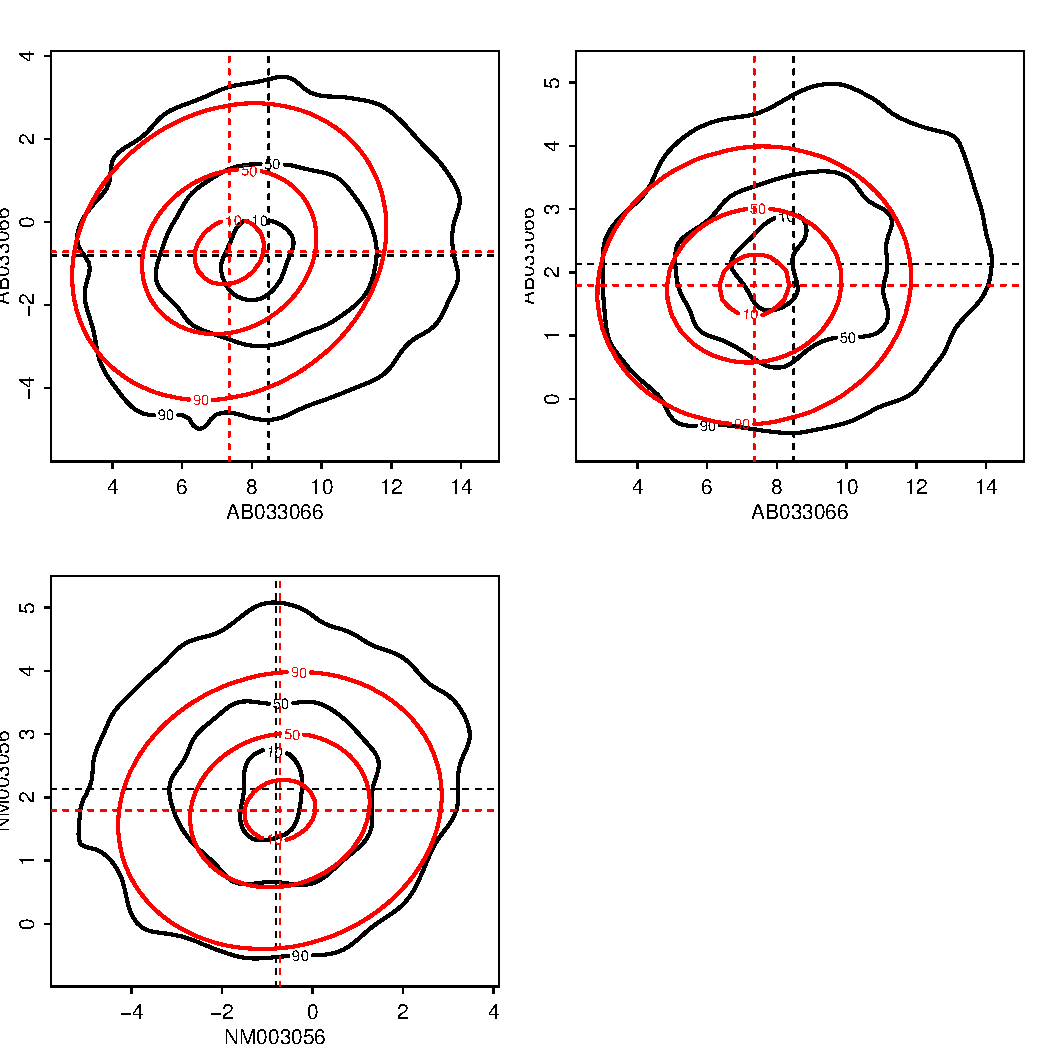
\includegraphics[width=.8\textwidth, height=.8\textheight]{\figfig/ISproposal-density2D}
  $$
}

%====================================================================
\subsection{Monte Carlo Markov chains (MCMC)}
\frame{\frametitle{Outline} \tableofcontents[currentsubsection]}
%====================================================================
\frame{ \frametitle{Limit distribution of Markov chain}

  \paragraph{Property.} If $\{\phibf^t\}_{t \geq 0}$ is an ergodic Markov chain (irreducible, aperiodic, ...) with
  \begin{itemize}
   \item initial distribution $\phibf^0 \sim \nu$,
   \item transition kernel $\phibf^t \gv \phibf^{t-1} \sim \kappa(\cdot \gv \phibf^{t-1})$:
  \end{itemize}
  $$
  p\left(\{\phibf^t\} \right) = \nu(\phibf^0) \times \kappa(\phibf^1 \gv \phibf^0) \times \kappa(\phibf^2 \gv \phibf^1) \times \kappa(\phibf^3 \gv \phibf^2) \times \dots
%   \prod_{t\geq 1} \kappa(\phibf^t \gv \phibf^{t-1})
  $$
  then
  \begin{itemize}
   \item it admits a \emphase{unique stationary distribution} $\mu$:
   $$
   \phibf^{t-1} \sim \mu \qquad \Rightarrow \qquad \phibf^t \sim \mu
   $$
   \item $\phibf^t$ converges towards $\mu$ in distribution
   $$
   \phibf^t \overset{\Delta}{\underset{t \rightarrow \infty}{\longrightarrow}} \mu
   $$
   for \emphase{any initial distribution} $\nu$
  \end{itemize}
}

%====================================================================
\frame{ \frametitle{Use for Bayesian inference}

  \paragraph{Aim.} Sample from
  $$
  p(\thetabf \gv \Ybf)
  $$
  
  \paragraph{Idea.} 
  \begin{itemize}
   \item Construct an ergodic Markov chain $\{\thetabf^t\}_{t \geq 0}$ with stationary distribution
   $$
   \mu(\thetabf) = p(\thetabf \gv \Ybf)
   $$
   \item Choose 'any' initial $\nu$ and simulate $\{\thetabf^t\}_{t \geq 0}$ \\ ~
   \item Until it 'reaches' its stationary distribution
  \end{itemize}
}

%====================================================================
\frame{ \frametitle{Metropolis-Hastings}

  \paragraph{Algorithm.} Define a shift kernel $\lambda(\cdot \gv \thetabf)$
  \begin{itemize}
   \item \pause Start with $\thetabf^0$
   \item \pause At step $t$, 
   \begin{enumerate}
    \item \pause sample $\thetabf' \sim \lambda(\cdot \gv \thetabf^{t-1})$;
   \item \pause compute the Metropolis-Hastings ratio (acceptance probability)
   $$
   \alpha(\thetabf', \thetabf^{t-1}) 
   = \frac{\lambda(\thetabf^{t-1} \gv \thetabf')}{\lambda(\thetabf' \gv \thetabf^{t-1})} \frac{p(\thetabf' \gv \Ybf)}{p(\thetabf^{t-1} \gv \Ybf)}
   \pause = \frac{\lambda(\thetabf^{t-1} \gv \thetabf')}{\lambda(\thetabf' \gv \thetabf^{t-1})} \frac{\pi(\thetabf') \ell(\Ybf \gv \thetabf')}{\pi(\thetabf^{t-1}) \ell(\Ybf \gv \thetabf^{t-1})};
   $$
   \item \pause $\text{set } \thetabf^t= \left\{
	 \begin{array}{ll}
	   \thetabf' & \text{with probability $\max(1, \alpha(\thetabf', \thetabf^{t-1}))$,} \\
	   \thetabf^{t-1} & \text{otherwise.}
	 \end{array} 
    \right.$
   \end{enumerate}
  \end{itemize}
  
  \bigskip \pause
  \paragraph{Properties.} 
  \begin{enumerate}
   \item $\lambda$ and $\alpha$ defined a Markov chain with stationary distribution $\mu(\thetabf) = p(\thetabf \gv \Ybf)$.
   \item If $\lambda(\cdot \gv \thetabf)$ is symmetric, $\alpha$ reduce to ${\pi(\thetabf') \ell(\Ybf \gv \thetabf')}/ [{\pi(\thetabf^{t-1}) \ell(\Ybf \gv \thetabf^{t-1})}]$
  \end{enumerate}
}

%====================================================================
\frame{ \frametitle{Metropolis-Hastings for logistic regression}

  \paragraph{Model.} 
  \begin{align*}
   \thetabf & \sim \pi(\thetabf) = \Ncal(\Obf_p, 100 \, \Ibf_p)\\
   \Ybf \gv \thetabf & \sim \ell(\Ybf \gv \thetabf) 
   = \prod_i \left(\frac{e^{\xbf_i^\intercal \thetabf}}{1 + e^{\xbf_i^\intercal \thetabf}}\right)^{y_i} \left(\frac{e^{\xbf_i^\intercal \thetabf}}{1 + e^{\xbf_i^\intercal \thetabf}}\right)^{1-y_i}
  \end{align*}

  \bigskip \bigskip \pause
  \paragraph{Algorithm settings.} 
  $$\thetabf^0 = \Obf_p$$
  $$\lambda( \cdot \gv \thetabf) = \Ncal(\Obf_p, .5 \, \Ibf_p)$$
}

%====================================================================
\frame{ \frametitle{M-H for logistic regression: R code}

  \pause
  \footnotesize{\tt 
  mu.prior = rep(0, p); Sigma.prior = 100*diag(p); Sigma.shift = .5*diag(p) \\ \pause
  theta.sample = matrix(0, M, p) \\ \pause
  theta.cur = theta.sample[1, ] \\ \pause
  logprior.cur = dmvnorm(theta.cur, mean=mu.prior, sigma=Sigma.prior, log=T) \\ \pause
  prob.cur = plogis(X\%*\%theta.cur) \\ \pause
  loglik.cur = sum(dbinom(Y, 1, prob.cur, log=T)) \\ \pause
  for (m in 2:M)\{ \\ \pause
  \qquad theta.tmp = rmvnorm(1, mean=theta.sample[m-1, ], sigma=Sigma.shift)[1, ] \\ \pause
  \qquad logprior.tmp = dmvnorm(theta.tmp, mean=mu.prior, sigma=Sigma.prior, log=T) \\ \pause
  \qquad prob.tmp = plogis(X\%*\%theta.tmp) \\ \pause
  \qquad loglik.tmp = sum(dbinom(Y, 1, prob.tmp, log=T)) \\ \pause
  \qquad alpha = exp(logprior.tmp + loglik.tmp - logprior.cur - loglik.cur) \\ \pause
  \qquad if(runif(1) < alpha)\{ \\ \pause
  \qquad \qquad theta.sample[m, ] = theta.tmp; \\ 
  \qquad \qquad logprior.cur = logprior.tmp; \\ 
  \qquad \qquad loglik.cur = loglik.tmp \\ \pause
  \qquad \qquad \}else\{ \\
  \qquad \qquad theta.sample[m, ] = theta.sample[m-1, ] \\
  \qquad \qquad \} \\ 
  \qquad \} \\ \pause
  \} \\
  }
}

%====================================================================
\frame{ \frametitle{Gibbs}

}

